\section{SOFTWARE}

\subsection{Description of the implementation}
The solution is implemented with a \acrfullr{fsm} with three states, starting from a TEST mode and switching to the next with the USER button of the L072CZ. A common factor of these states is that in all of them, all the data from the sensors need to be obtained.

To solve the need for asynchronous data obtention from the sensors, the solution is based on threads and queues. There are three threads:
\begin{itemize}
    \item Main thread with the \acrshort{fsm}.
    \item I2C thread.
    \item GPS thread.
\end{itemize}

These thread are signalized to wake up when new measurements are needed by the \acrshort{fsm}. When all the information is collected, the information goes to the main thread through a Mbed-OS queue. When all the necessary 
information is obtained, the main thread sends the new data to the computer and waits a set amount of time to start the process again.
\subsection{Module, threads and communications design}
To make the design modular, each hardware element is implemented in a single module, with a \texttt{.cpp} and a \texttt{.h} file.

Considering the asynchronous nature of some of the sensors, the i2c sensors were implemented in an independent thread and the GPS in another thread. In the , the final module design as well as the threads implemented 
can be seen in \autoref{fig:moduleDiagram}.
\begin{figure}[H]
    \centering
    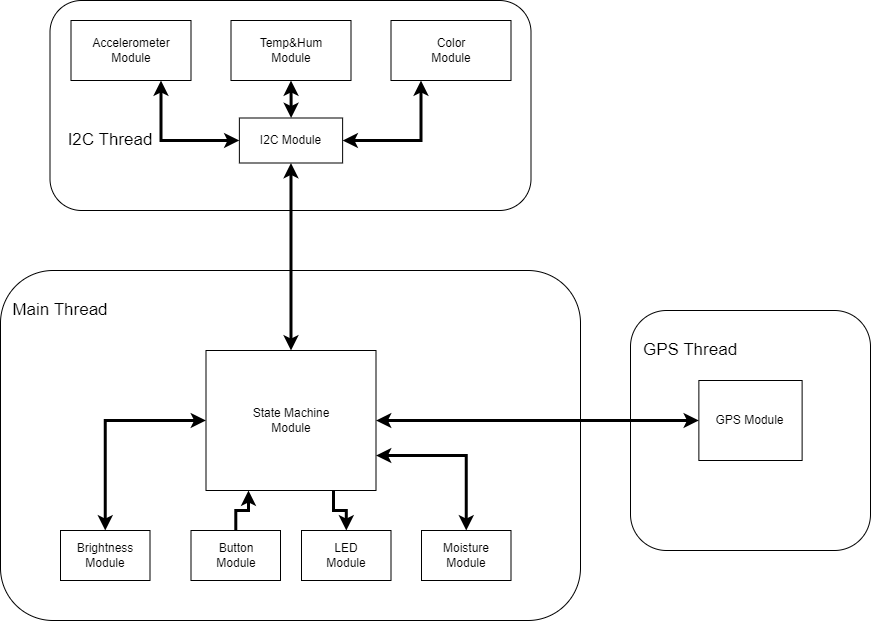
\includegraphics[width=0.9\textwidth]{images/4/softdiagram.png}
    \caption{Module diagram of the software and threads}
    \label{fig:moduleDiagram}
\end{figure}

For the communications from the control to the \acrshort{i2c} and the GPS, there was only need to indicate to the \acrshort{i2c} and GPS threads to launch all the necessary measurements on demand, so in this case signals were used.
For the data flowing from the sensors to the control module, as signals in a processor are limited(in our case 32 bit register for signals), a queue was used.

A queue is a thread safe mechanism of low level that implements a FIFO buffer with a in endpoint and an out endpoint. Any process can insert new data into the queue with a blocking call and the same can be done to extract the data. Finally, the data 
inside the queue is managed by the queue itself(at least in the implementation in Mbed-OS).

To reduce the memory usage, only one queue was defined for the whole system. With this done, extra logic was needed to differentiate messages from different sensors, so a message structure was defined like a pseudo-protocol. This can be seen in the \hyperref[appendix]{appendix}.

\subsection{State machine module}
At the start of the system, the main calls for the initialization of all the modules. This is important because the creation of the I2C and GPS threads take some time. When this is done, the main initializes the state machine 
and enters a loop to do a cycle of the state machine.

The state machine includes two timeouts that are configured for each state, depending on the needs.
\begin{itemize}
    \item The first timeout is configured as the time needed between sending the information to the computer.
    \item For the second timeout, the configuration is to make it generate an interruption \texttt{400 ms} earlier. When this happens, the controller sends signals for every thread. This signal enforces the reading of new 
    measurements.
\end{itemize}
When the signals are sent, the main thread is sent to sleep \texttt{400 ms}, at that time, it wakes up and analyzes all the data that has been sent to the queue. This time was selected as a time to let the other threads collect all the necessary data.

When all the messages are collected, the data is processed depending on the state of the system:
\begin{itemize}
    \item TEST mode: as the requirements specify, the data is formatted and sent to the computer as in \autoref{fig:testSerial}. Depending on the highest color component, the RGB led changes accordingly.
    \begin{figure}[H]
        \centering
        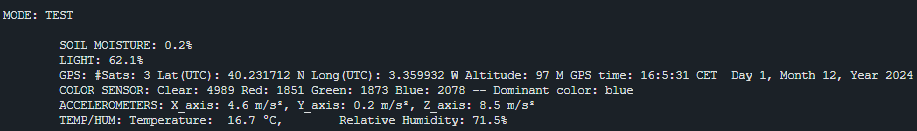
\includegraphics[width=0.9\textwidth]{images/4/TestSerial.png}
        \caption{Information sent to the computer in the TEST mode}
        \label{fig:testSerial}
    \end{figure}
    \clearpage
    \item NORMAL mode: as the requirements specify, the time the messages are read, maximum values and mean values are calculated, as well as situations like extreme moisture.
    
    All the limitations are in the \autoref{Limits}.

    \begin{table}[H]
        \begin{center}
            \begin{tabular}{|p{0.20\textwidth} | p{0.20\textwidth} | p{0.20\textwidth}| p{0.20\textwidth}|}
                \hline
                \textbf{Parameter} & \textbf{High limit} & \textbf{Low limit} & \textbf{Led color}\\
                \hline
                Temperature & 35 & 10 & red \\
                \hline
                Humidity & 75 & 25 & blue \\
                \hline
                Brightness & 80 & 10 & Yellow \\
                \hline
                Moisture & 85 & 5 & Purple \\
                \hline
                Color & Blue &  & White \\
                \hline
            \end{tabular}
        \end{center}
        \caption{Limits defined for the parameters in the NORMAL mode}
        \label{Limits}
    \end{table}

    All of this information is sent to the computer, and when one hour has passed, the maximum and mean values are also sent. The format is presented in \autoref{fig:normalSerial}.
    \begin{figure}[H]
        \centering
        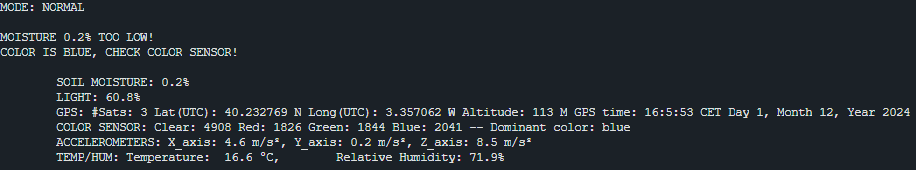
\includegraphics[width=0.9\textwidth]{images/4/NormalSerial.png}
        \caption{Information sent to the computer in the NORMAL mode}
        \label{fig:normalSerial}
    \end{figure}

    \item ADVANCED mode: this mode is presented and described in it's own \hyperref[AdvancedChapter]{chapter}.
\end{itemize}

Finally, the USER button allows for switching modes in a circular way. When this button is pressed:
\begin{enumerate}
    \item The timeouts are re-configured.
    \item The led of the board that is on changes to indicate the new state.
    \item The RGB led is turned off.
    \item The thread waits \texttt{400 ms} for any new messages from the other threads, in order to empty the queue for the new state.
\end{enumerate}

As a final note, as this state machine is working under the main thread of Mbed-OS, no changes were done to the stack or any other property of this thread.
\clearpage
\subsection{I2C module}

The \acrshort{i2c} module controls the measurement of the accelerometer, temperature and humidity and color sensors.

As there are three different sensors with different requirements, at the initialization of the I2C thread, all the sensors are started sequentially, using a global I2C object. It must be noted that as all the sensors 
support it, the I2C is used with a frequency of \texttt{400 kHz}.

For the initialization, the next steps are done:
\begin{itemize}
    \item \textbf{Initialization of the accelerometer}: first the accelerometer is reseated, when this finish, the dynamic configuration is set to 8G, this is because the use case doesn't need that much high sensibility.
    \item \textbf{Initialization of the color sensor}: for the color sensor, the dataset specifies a different approach with a command register. In this case, this sensor is configured to remove any wait state, this is done because 
    the sensor has a limit of wait time less that 30 seconds, so the readings are done on demand, this is by turning on and off the sensor. Lastly, the sensor is configured with an integration time of \texttt{154 ms}.
\end{itemize}

When all the configuration is done, the thread enters a loop where it waits for an \texttt{I2C\_SIGNAL} from the state machine. Once this happens, the flag is cleared and the next steps happen:
\begin{enumerate}
    \item Reading of the accelerometer data, conversion of the data and queue acceleration message sent.
    \item Powering the color sensor, waiting for the integration time and reading of the data to send the color message. Power off the sensor.
    \item Force a reading of humidity and temperature, converting values as told in the dataset\cite{Support_Documents_TechnicalDocs_Si7021A20}.
\end{enumerate}

To finalize, the thread goes back to wait for another signal from the state machine.
\clearpage
\subsection{GPS module}
The GPS module implements the GPS thread and focuses on obtaining and parsing the data from the GPS chip.

The GPS is constantly sending data to the serial connection in a baud rate of \texttt{9600}. To read this data, when the thread wakes from a \texttt{GPS\_SIGNAL}, the thread is constantly reading the characters obtained in the \acrshort{uart} and adding them to a 
buffer. If the next character is a new line character, the buffer is sent to the parse\_gps\_sentence function.

For this parsing, as the system only needs the location, time and data, the parsing is only done to specific sentences of the \acrshort{nmea} data format in \autoref{fig:nmeaSentences}.
\begin{figure}[H]
    \centering
    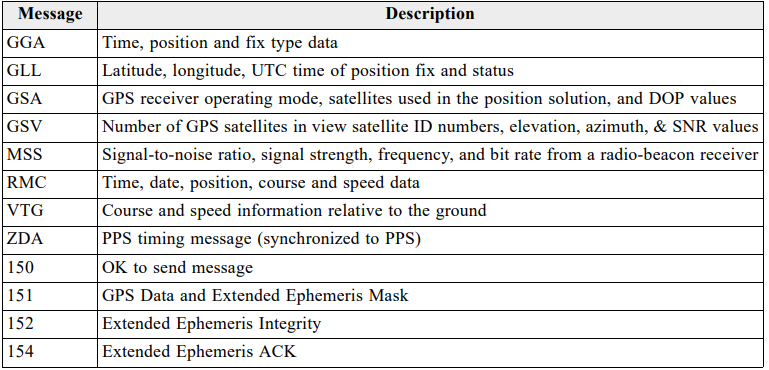
\includegraphics[width=0.9\textwidth]{images/4/nmea.png}
    \caption{NMEA possible sentences\cite{NMEAReferenceManual}}
    \label{fig:nmeaSentences}
\end{figure}
In this use case, the GPS thread only searches for:
\begin{itemize}
    \item \textbf{GGA}: contains the information about the actual time, latitude, longitude, altitude and number of satellites detected.
    \item \textbf{RMC}: contains information about the actual time, the actual date and other data that the system doesn't use.
\end{itemize}
To parse the sentences, the function \texttt{strncmp} was used to analyze the sentence type and \texttt{sscanf} to parse all the information like a pseudo-regex.

When both sentences are found, the message for the queue is built and inserted, finally, the GPS thread goes back to wait for a new signal from the state machine.

\clearpage
\subsection{Code size}
For the code size of the project, the information resulting from the compilation in Mbed Studio is presented in the next figures. It must be noted that no changes to the default compilation profiles were done.
\begin{figure}[H]
    \centering
    \begin{subfigure}[t]{0.45\textwidth}
        \centering
        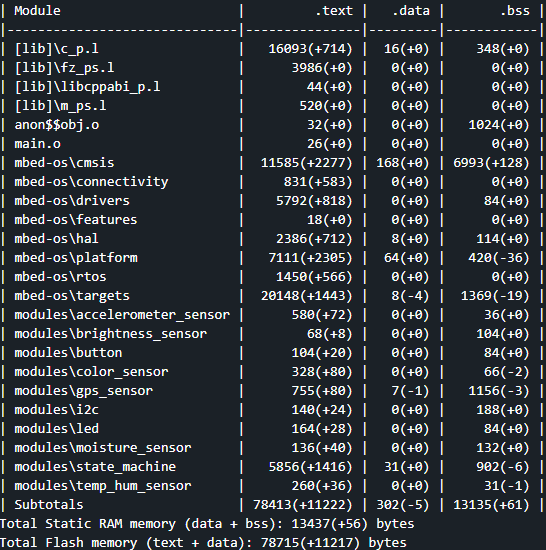
\includegraphics[width=0.95\textwidth]{images/4/Debug.png}
        \caption{Debug compilation}
    \end{subfigure}
    \begin{subfigure}[t]{0.45\textwidth}
        \centering
        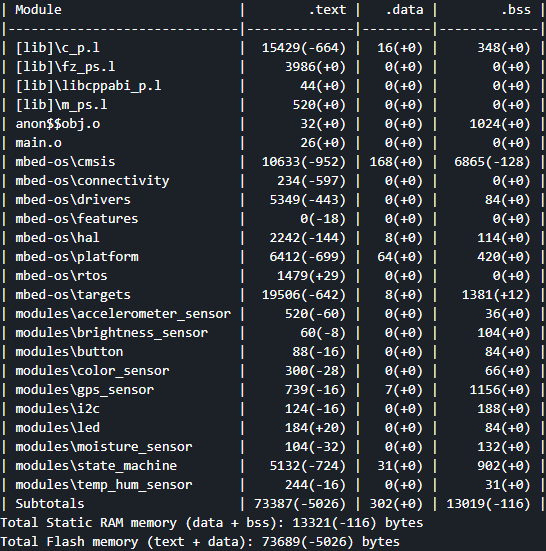
\includegraphics[width=0.95\textwidth]{images/4/Develop.png}
        \caption{Develop compilation}
    \end{subfigure}
    \begin{subfigure}[t]{0.45\textwidth}
        \centering
        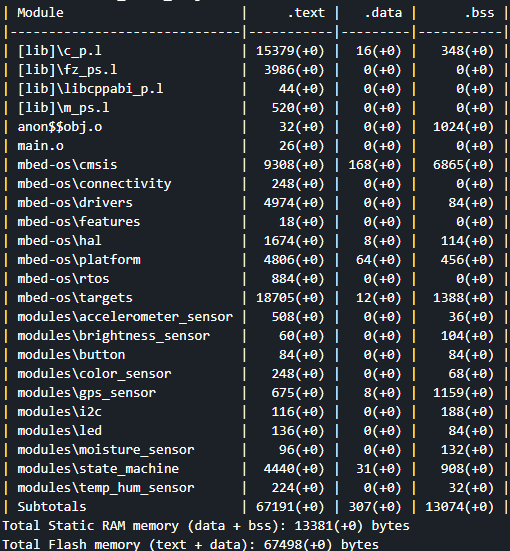
\includegraphics[width=0.95\textwidth]{images/4/Release.png}
        \caption{Release compilation}
    \end{subfigure}
    \caption{Code size and module size for every compilation profile}
    \label{fig:compilation}
\end{figure}

The most heavy modules in terms of size were:
\begin{enumerate}
    \item The state machine with 476 lines of code.
    \item The GPS with 86 lines of code, but with a parsing of a string, which needs lot of resources.
\end{enumerate}
